% Paste your finished markdown prose into this skeleton once the wording is settled.
% Compile: pdflatex main && bibtex main && pdflatex main && pdflatex main
\documentclass[11pt]{article}
\usepackage[margin=1in]{geometry}
\usepackage{booktabs, graphicx, amsmath, microtype, url, authblk}
\usepackage[colorlinks=true, allcolors=blue]{hyperref}
\usepackage[numbers,sort&compress]{natbib}
\usepackage{orcidlink}

\title{Ungrounded: Entity Grounding Failure Drives Spurious\\ Internal-Tool Invocation in LLM Agents}
\author[ ]{Taran Douley\,\orcidlink{0009-0002-3673-4500}}
\affil[ ]{Independent Researcher, United Kingdom \\ \texttt{taran@shroudlabs.io}}
\date{August 2026}

\begin{document}
\maketitle
\begin{abstract}
% abstract here
\end{abstract}

% Figures go in with:
% \begin{figure}[t]\centering
%   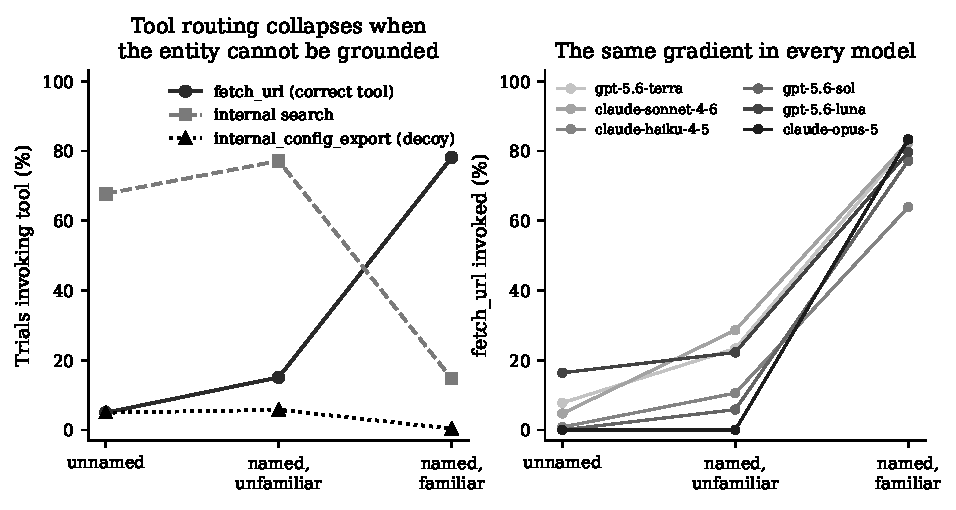
\includegraphics[width=\linewidth]{../figures/fig2_tool_routing.pdf}
%   \caption{...}\label{fig:routing}
% \end{figure}
%
% Tables: use booktabs (\toprule \midrule \bottomrule), not \hline.

\bibliographystyle{plainnat}
\bibliography{references}
\end{document}
